\documentclass[professionalfont,10pt]{beamer}

\useinnertheme{rectangles}
\beamertemplatenavigationsymbolsempty
\addtobeamertemplate{navigation symbols}{}{%
    \usebeamerfont{footline}
    \usebeamercolor[fg]{footline}
    \hspace{5mm}
    \insertframenumber/\inserttotalframenumber
}
\usecolortheme{seahorse}
\setbeamercolor{alerted text}{fg=white!20!blue!30!red}
\setbeamercolor{footline}{fg=black}
\setbeamersize{text margin left=5mm,text margin right=5mm}

\usepackage{bbm}
\usepackage{booktabs}
\usepackage{mathtools}
\usepackage{tikz,tikzpeople}
\usepackage{pgfplots}
\usepackage[outline]{contour}
\contourlength{1.2pt}

\usepackage{graphicx}
\usepackage{animate}

\usepackage{threeparttable}

\begin{filecontents}{decision_practice_timeline.txt}
*::0
::1
::2
::1
::2
::1
::2
::1
*::3
::1
::2
::1
::2
::1
::2
*::4
*::5
\end{filecontents}

\begin{filecontents}{implement_practice_timeline.txt}
*::0
::1
::2
::3
::4
::5
::1
::2
::3
::4
::5
::1
*::6
*::7
\end{filecontents}

\title{Temptation: Immediacy and Certainty}
\author{Lucas Reddinger}
\institute{UCSB}
\date{11 November 2020}

\begin{document}

\frame{\titlepage}

\begin{frame}{Motivation and question}
\begin{itemize}[<+->]
\item Ever make long-term goals, then fail to follow your plan?
\item Often choose a short-term temptation: dynamically inconsistent behavior
\vfill
\item \alert{Is an option less tempting when its consequence is uncertain?}
\vfill
\item Time preferences, risk preferences, and their relationship are foundational to economics
\vfill
\item I study how a \alert{preference for immediacy} is affected by \alert{uncertainty}
\end{itemize}
\end{frame}

\begin{frame}{Motivating example}{Keren and Roelofsma (1995)}
\begin{itemize}
    \item Decide between a smaller reward or a larger delayed reward
    \vspace{2\baselineskip}
    \pause
    \item Choose one:\uncover<6->{\hfill \alert{\textbf{If coin-flip is heads:}} \hspace{4em} \phantom{.}}
    \begin{itemize}
      \item \$50 today \uncover<4->{\hfill \alert{\emph{modal}} \hspace{16em} \phantom{\emph{modal} .}}
      \item \$55 in 1 month \uncover<7->{\hfill \alert{\emph{modal}} \hspace{12em} \phantom{.}}
    \end{itemize}
    \pause
    \item Choose one:
    \begin{itemize}
      \item \$50 in 5 months
      \item \$55 in 6 months \uncover<5->{\hfill \alert{\emph{modal}} \hspace{4em}} \uncover<7->{\alert{\emph{modal}} \hspace{12em} \phantom{.}}
    \end{itemize}
    \vspace{2\baselineskip}
    \item<8-> The preference for immediacy is eliminated by uncertainty
    \item<9-> Little or no immediacy effect if consequence probability is $0.5$ or $0.9$
\end{itemize}
\end{frame}

\begin{frame}{Some evidence of risk affecting patience}
\begin{itemize}
\item<1-> Hypothetical consequences:
\begin{itemize}
\item<2-> Keren and Roelofsma (1995) \textcolor{gray}{-- results for the previous slide}
\item<3-> Weber and Chapman (2005)
\end{itemize}
\vspace{2em}
\item<4-> Almost-hypothetical consequences:
\begin{itemize}
\item <5->Baucells and Heukamp (2010) \uncover<6->{-- each decision paid with prob. $0.0008$ }
\end{itemize}
\vspace{2em}
\item<7-> These suggest highly-likely consequences necessary for present bias
\item<8-> Yet to be tested using certain (or even somewhat likely) consequences
\end{itemize}
\end{frame}

\begin{frame}{Background: Exponentially Discounted Utility model}{Samuelson (1937)}
$$U_t = \sum_{\tau=0} \delta^\tau u(c_{t+\tau})$$
\vspace{2\baselineskip}
\begin{itemize}
\item<2-> Consumption utility flow $u(c_{t+\tau})$ at time ${t+\tau}$
\vspace{1\baselineskip}
\item<3-> Constant discount factor: $0\leq \delta \leq 1$
\end{itemize}
\end{frame}

\begin{frame}{Background: dynamic consistency}
  \begin{itemize}
    \item[(a)] Value on Day 1: $U_1 = u(c_1) + \delta u(c_2) + \delta^2 u(c_3)$
    \item[(b)]<3-> Value on Day 2: $U_2 = u(c_2) + \delta u(c_3)$
    \item<5-> \alert{Plan of action is consistent over time}
  \end{itemize}
  \vspace{1\baselineskip}
  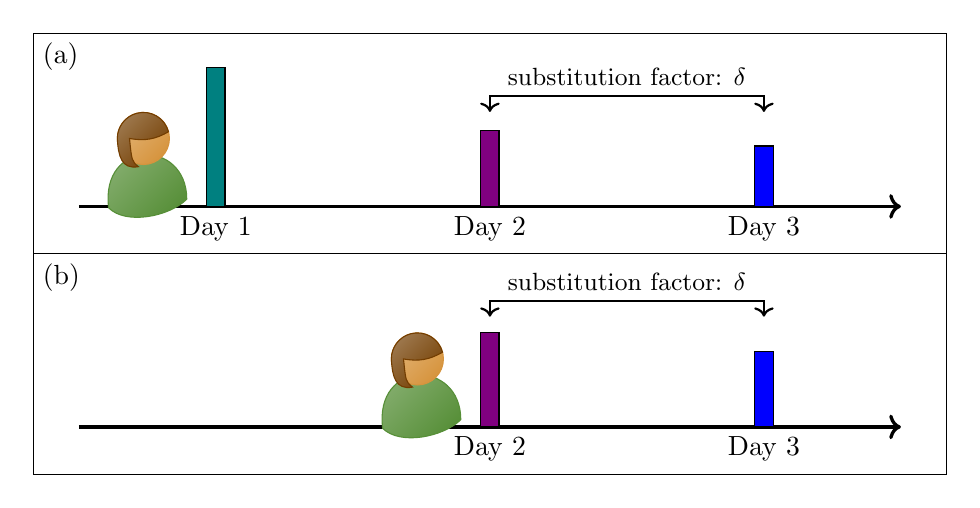
\begin{tikzpicture}[xscale=0.58,yscale=0.4]
    \draw[white,line width=4pt] (5,1.5) rectangle (25,15.5);    
    \draw[black] (5,8.5) rectangle (25,15.5);
    \node[black, below right] at (5,15.5) {(a)};
    \draw[->,black,very thick] (6,10) -- (24,10);
    \node[person,female,saturated,minimum size=1cm,yshift=15pt] at (7.5,10) {};
    \draw[-,preaction={fill=teal}] (8.8,14.4) rectangle (9.2,10);
    \draw[] (9.0,10) node[below] {Day 1};
    \draw[-,preaction={fill=violet}] (14.8,12.4) rectangle (15.2,10);
    \draw[] (15.0,10) node[below] {Day 2};
    \draw[-,preaction={fill=blue}] (20.8,11.92) rectangle (21.2,10);
    \draw[] (21.0,10) node[below] {Day 3};
    \draw<2->[<->,black,thick] (15,13) -- (15,13.5) -- (18,13.5) node[above] {\small substitution factor: $\delta$} -- (21,13.5) -- (21,13);
    \draw<3->[black] (5,1.5) rectangle (25,8.5);
    \node<3->[black, below right] at (5,8.5) {(b)};
    \draw<3->[->,black,very thick] (6,3) -- (24,3);
    \node<3->[person,female,saturated,minimum size=1cm,yshift=15pt] at (13.5,3) {};
    \draw<3->[-,preaction={fill=violet}] (14.8,6) rectangle (15.2,3);
    \draw<3->[] (15.0,3) node[below] {Day 2};
    \draw<3->[-,preaction={fill=blue}] (20.8,5.4) rectangle (21.2,3);
    \draw<3->[] (21.0,3) node[below] {Day 3};
    \draw<4->[<->,black,thick] (15,6.5) -- (15,7) -- (18,7) node[above] {\small substitution factor: $\delta$} -- (21,7) -- (21,6.5);
  \end{tikzpicture}
\end{frame}

\begin{frame}{Background: Quasi-Hyperbolic Discounting}{Laibson (1997)}
$$U_t = u(c_t) + \sum_{\tau=1} \beta \delta^\tau u(c_{t+\tau})$$
\vspace{2\baselineskip}
\begin{itemize}
\item<2-> Consumption utility flow $u(c_{t+\tau})$ at time ${t+\tau}\in\mathbb{N}$
\vspace{1\baselineskip}
\item<3-> Constant discount factor $0\leq \delta \leq 1$
\vspace{1\baselineskip}
\item<4-> Also discount all future periods by factor $0 \leq \beta \leq 1$
\vspace{1\baselineskip}
\item<5-> Gives a preference for immediacy (present bias) if $\beta<1$
\end{itemize}
\end{frame}

\begin{frame}{Background: present bias}
  \begin{itemize}
    \item[(a)] Value on Day 1: $U_1 = u_1 + \beta \delta u_2 + \beta \delta^2 u_3$
    \item[(b)]<3-> Value on Day 2: $U_2 = u_2 + \beta \delta u_3$
    \item<5-> \alert{Plan of action changes for immediate consumption}
  \end{itemize}
  \vspace{1\baselineskip}
  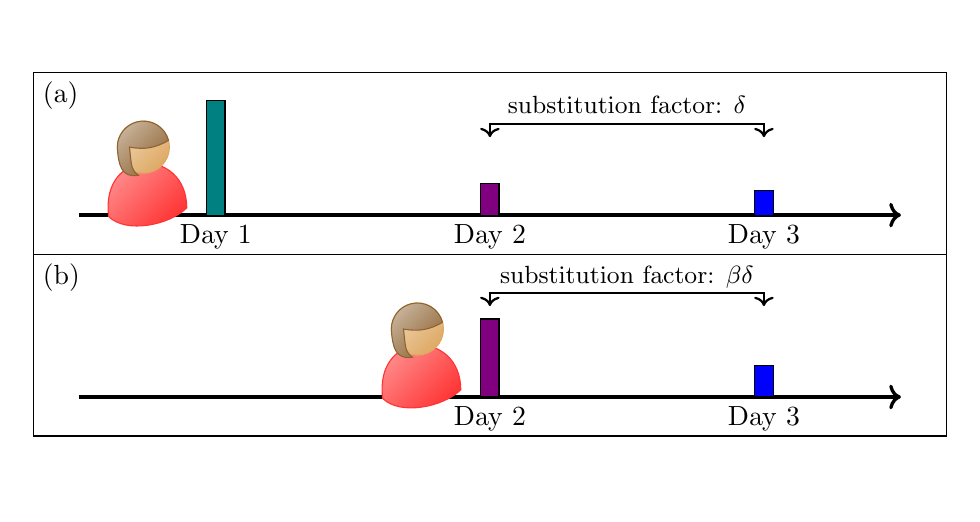
\begin{tikzpicture}[xscale=0.58,yscale=0.33]
    \draw[white,line width=4pt] (5,-0.5) rectangle (25,17);
    \draw[black] (5,8.5) rectangle (25,15.5);
    \node[black, below right] at (5,15.5) {(a)};
    \draw[->,black,very thick] (6,10) -- (24,10);
    \node[person,female,shirt=red,minimum size=1cm,yshift=15pt] at (7.5,10) {};
    \draw[-,preaction={fill=teal}] (8.8,14.4) rectangle (9.2,10);
    \draw[] (9.0,10) node[below] {Day 1};
    \draw[-,preaction={fill=violet}] (14.8,11.2) rectangle (15.2,10);
    \draw[] (15.0,10) node[below] {Day 2};
    \draw[-,preaction={fill=blue}] (20.8,10.96) rectangle (21.2,10);
    \draw[] (21.0,10) node[below] {Day 3};
    \draw<2->[<->,black,thick] (15,13) -- (15,13.5) -- (18,13.5) node[above] {\small substitution factor: $\delta$} -- (21,13.5) -- (21,13);
    \draw<3->[black] (5,1.5) rectangle (25,8.5);
    \node<3->[black, below right] at (5,8.5) {(b)};
    \draw<3->[->,black,very thick] (6,3) -- (24,3);
    \node<3->[person,female,shirt=red,minimum size=1cm,yshift=15pt] at (13.5,3) {};
    \draw<3->[-,preaction={fill=violet}] (14.8,6) rectangle (15.2,3);
    \draw<3->[] (15.0,3) node[below] {Day 2};
    \draw<3->[-,preaction={fill=blue}] (20.8,4.2) rectangle (21.2,3);
    \draw<3->[] (21.0,3) node[below] {Day 3};
    \draw<4->[<->,black,thick] (15,6.5) -- (15,7) -- (18,7) node[above,yshift=-2pt] {\small substitution factor: $\beta \delta$} -- (21,7) -- (21,6.5);
  \end{tikzpicture}
\end{frame}

\begin{frame}{Methodology: timing of utility flows}
\begin{itemize}[<+->]
\item DU and QHD model \alert{consumption (utility) flows}
\item Monetary payments unlikely to demonstrate present bias
\vspace{1\baselineskip}
\item Any liquidity suggests that the timing of monetary payments will differ from resultant consumption timing
\vspace{1\baselineskip}
\item Augenblick, Neiderle, and Sprenger (2015) estimate present bias
\begin{itemize}[<+->]
\item For money: $\hat\beta_\text{money}=0.974, \;\text{SE}=0.009$
\item For effort: $\hat\beta_\text{effort}=0.888, \;\text{SE}=0.033$
\end{itemize}
\vspace{1\baselineskip}
\item Imai, Rutter, Camerer (2020) review $220$ present bias estimates
\begin{itemize}[<+->]
\item For money: $\bar{\beta}_\text{money}=0.9943, \;\text{SE}=0.0020$
\item For effort: $\bar{\beta}_\text{effort}=0.9072, \;\text{SE}=0.0242$
\end{itemize}
\vspace{1\baselineskip}
\item This literature uses substantial risk (e.g., $1/20$) to incentivize decisions
\end{itemize}
\end{frame}

\begin{frame}{Methodology}
\begin{itemize}[<+->]
\item Unpleasant real-effort task that subjects want to smooth across days
\item Subjects choose how many real-effort tasks to delay
\item Make choices at various price ratios
\vspace{1\baselineskip}
\item Choose 2 days before work
\item Choose again on the first workday
\item Vary how these decisions are incentivized between treatments
\vspace{1\baselineskip}
\item How does the incentive mechanism affect present bias factor $\beta$?
\end{itemize}
\end{frame}

\begin{frame}{Contribution}
\begin{itemize}[<+->]
\item \alert{Questions:}
\begin{itemize}[<+->]
\item Does uncertainty help people follow their plans?
\item Does certainty make an option more tempting?
\end{itemize}
\vspace{1\baselineskip}
\item \alert{Methodology:}
\begin{itemize}[<+->]
\item Is present bias factor $\beta$ moderated by risk?
\item Use decisions that are risk-free (they matter with \emph{certainty})
\item Use consequences that are immediate (real-effort required \emph{now})
\end{itemize}
\vspace{1\baselineskip}
\item \alert{Summary of findings:}
\begin{itemize}[<+->]
\item Individuals are far more present-biased if decisions are certainty implemented
\item Similar proportion of present-biased individuals; their bias is more severe
\item $\hat\beta = 0.93$ under risk, but $\hat\beta = 0.69$ under certainty
\end{itemize}
\end{itemize}
\end{frame}

\begin{frame}{Roadmap}
\begin{itemize}[<+->]
\item Experimental design
\begin{itemize}[<+->]
\item Overview
\item Details for baseline treatment
\item Treatment differences
\end{itemize}
\item Results
\begin{itemize}[<+->]
\item Subject recruitment and retention
\item Non-parametric results
\item Introduce model
\item Parametric results
\item Robustness
\end{itemize}
\item Conclusion
\end{itemize}
\end{frame}

\begin{frame}
\vfill
\begin{center}
{\Large Experimental design}
\end{center}
\vfill
\end{frame}

\begin{frame}{Experimental design: overview}
\begin{itemize}
\item Longitudinal experiment conducted on Amazon Mechanical Turk
\end{itemize}
\resizebox{\textwidth}{!}{
  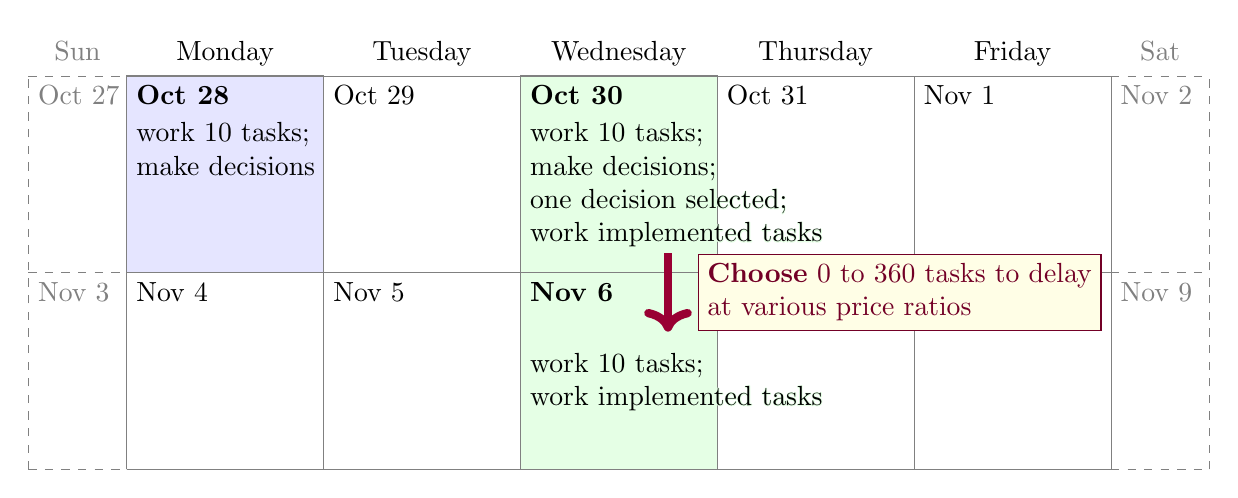
\begin{tikzpicture}[domain=0:7, scale=2.5]
    \draw[very thin,color=white!1] (-0.5,0) rectangle (5.5,2);
    \pause{}
    \draw[very thin,color=black!50] (0,0) grid (5,2);
    \draw[very thin,color=black!50,fill=green!10] (2,0) grid (3,2) rectangle (2,0);
    \draw[very thin,color=black!50,fill=blue!10] (0,1) grid (1,2) rectangle (0,1);
    \draw[very thin,color=black!50,dashed] (5,0) grid[xstep=.5,ystep=1] (5.5,2);
    \draw[very thin,color=black!50,dashed] (-0.5,0) grid[xstep=.5,ystep=1] (0,2);
    \draw[] (-0.25,2) node[above, yshift=-0.15em, color=black!50] {Sun\strut};
    \draw[] (0.5,2)  node[above, yshift=-0.15em] {Monday\strut};
    \draw[] (1.5,2)  node[above, yshift=-0.15em] {Tuesday\strut};
    \draw[] (2.5,2)  node[above, yshift=-0.15em] {Wednesday\strut};
    \draw[] (3.5,2)  node[above, yshift=-0.15em] {Thursday\strut};
    \draw[] (4.5,2)  node[above, yshift=-0.15em] {Friday\strut};
    \draw[] (5.25,2) node[above, yshift=-0.15em, color=black!50] {Sat\strut};
    \draw[] (-0.5,2) node[below right, align=left,color=black!50] {Oct 27};
    \draw[] (0,2) node[below right, align=left] { \textbf{Oct 28} };
    \draw[] (1,2) node[below right, align=left] {Oct 29};
    \draw[] (2,2) node[below right, align=left] { \textbf{Oct 30} };
    \draw[] (3,2) node[below right, align=left] {Oct 31};
    \draw[] (4,2) node[below right, align=left] {Nov 1};
    \draw[] (5,2) node[below right, align=left, color=black!50] {Nov 2};
    \draw[] (-0.5,1) node[below right, align=left, color=black!50] {Nov 3};
    \draw[] (0,1) node[below right, align=left] {Nov 4};
    \draw[] (1,1) node[below right, align=left] {Nov 5};
    \draw[] (2,1) node[below right, align=left] { \textbf{Nov 6} };
    \draw[] (3,1) node[below right, align=left] {Nov 7};
    \draw[] (4,1) node[below right, align=left] {Nov 8};
    \draw[] (5,1) node[below right, align=left, color=black!50] {Nov 9};
    \draw[<-,black!20!purple,line width=3pt] (2.75,0.70) -- (2.75,1.10);
    \draw[] (2.9,0.9) node[draw, thin, color=black!40!purple, fill=yellow!10, right, align=left] {\textbf{Choose} 0 to 360 tasks to delay \\ at various price ratios};
    \pause{}
    \draw[] (0,2) node[below right, align=left] { \strut \\ work 10 tasks; };
    \pause{}
    \draw[] (0,2) node[below right, align=left] { \strut \\ \strut \\ make decisions};
    \pause{}
    \draw[] (2,2) node[below right, align=left] { \strut \\ work 10 tasks; };
    \pause{}
    \draw[] (2,2) node[below right, align=left] { \strut \\ \strut \\ make decisions; };
    \pause{}
    \draw[] (2,2) node[below right, align=left] { \strut \\ \strut \\ \strut \\ \contour{green!10}{one decision selected;} };
    \pause{}
    \draw[] (2,2) node[below right, align=left] { \strut \\ \strut \\ \strut \\ \contour{green!10}{\strut} \\ \contour{green!10}{work implemented tasks} };
    \pause{}
    \draw[] (2,1) node[below right, align=left] { \strut \\ \strut \\ work 10 tasks; };
    \pause{}
    \draw[] (2,1) node[below right, align=left] { \strut \\ \strut \\ \strut \\ \contour{green!10}{work implemented tasks} };
    \pause{}
  \end{tikzpicture}
}
\begin{itemize}[<+->]
\item First session: \$1.50 \hspace{3em} Second: \$1.50  \hspace{3em} Third: \$6.50
\item Subjects removed upon failure to complete a day's session
\item Ten decisions total: \alert{treatments vary probability of implementation}
\end{itemize}
\end{frame}

\begin{frame}{Real-effort task}
\centering\fbox{\animategraphics[scale=0.3,trim=0cm 14cm 12cm 0cm,step]{15}{animate_frames/task_practice}{0}{2}}
\end{frame}

\begin{frame}{Treatment: \alert{risky price, risky day} (baseline)}
\begin{itemize}[<+->]
\item Allocate real effort between Day 2 and Day 9
\begin{itemize}[<+->]
\item $e_i^\text{Day 2} + R_i e_i^\text{Day 9} = 360$
\item Choose for each possible trade-off rate (price) $R_i \in \{1.5, 1.25, 1, 0.75, 0.5\}$
\end{itemize}
\item Decide on Day 0 and then again on Day 2\\
\vspace{1\baselineskip}
\begin{tabular}{ll}
\hline
Day 0 & \uncover<5->{ Day 2 } \\ \hline
Allocate at $R_1$ (prob 1/10) & \uncover<5->{ Allocate at $R_1$ (prob 1/10) } \\
Allocate at $R_2$ (prob 1/10) & \uncover<5->{ Allocate at $R_2$ (prob 1/10) } \\
Allocate at $R_3$ (prob 1/10) & \uncover<5->{ Allocate at $R_3$ (prob 1/10) } \\
Allocate at $R_4$ (prob 1/10) & \uncover<5->{ Allocate at $R_4$ (prob 1/10) } \\
Allocate at $R_5$ (prob 1/10) & \uncover<5->{ Allocate at $R_5$ (prob 1/10) } \\ \hline
\end{tabular}
\end{itemize}
\end{frame}

\begin{frame}
\centering\fbox{\animategraphics[scale=0.3,trim=0cm 11cm 6cm 0cm,step]{10}{animate_frames/allocate_practice}{0}{19}}
\end{frame}

\begin{frame}
\centering\fbox{\animategraphics[scale=0.25,trim=0cm 4.5cm 4cm 0cm,timeline=decision_practice_timeline.txt]{5}{animate_frames/decision_practice}{}{}}
\end{frame}

\begin{frame}
\centering\fbox{\animategraphics[scale=0.3,trim=0cm 20cm 8cm 0cm,timeline=implement_practice_timeline.txt]{6}{animate_frames/implement_practice}{}{}}
\end{frame}

\begin{frame}
\centering\fbox{\animategraphics[scale=0.3,trim=0cm 12.5cm 12cm 0cm,step]{15}{animate_frames/task_implemented_practice}{0}{2}}
\end{frame}

\begin{frame}{Treatment: \alert{risky price, certain day}}
\begin{itemize}
\item Allocate real effort between Day 2 and Day 9
\begin{itemize}
\item $e_i^\text{Day 2} + R_i e_i^\text{Day 9} = 360$
\item Choose for each possible trade-off rate (price) $R_i \in \{1.5, 1.25, 1, 0.75, 0.5\}$
\end{itemize}
\item Decide on Day 0 and then again on Day 2\\
\vspace{1\baselineskip}
\begin{tabular}{ll}
\hline
Day 0 & \uncover<3->{ Day 2 } \\ \hline
Allocate at $R_1$ (prob 1/10) & \uncover<3->{ Allocate at $R_1$ (prob \alert{1/5}) } \\
Allocate at $R_2$ (prob 1/10) & \uncover<3->{ Allocate at $R_2$ (prob \alert{1/5}) } \\
Allocate at $R_3$ (prob 1/10) & \uncover<3->{ Allocate at $R_3$ (prob \alert{1/5}) } \\
Allocate at $R_4$ (prob 1/10) & \uncover<3->{ Allocate at $R_4$ (prob \alert{1/5}) } \\
Allocate at $R_5$ (prob 1/10) & \uncover<3->{ Allocate at $R_5$ (prob \alert{1/5}) } \\ \hline
\end{tabular}
\vspace{1\baselineskip}
\uncover<2->{ \item Just before Day 2 decisions, informed that a coin flip has selected only Day 2 decisions to matter }
\uncover<4->{ \item One of these \alert{five} decisions is implemented randomly}
\end{itemize}
\end{frame}

\begin{frame}{Treatment: \alert{certain price, risky day}}
\begin{itemize}
\item Allocate real effort between Day 2 and Day 9
\begin{itemize}
\item $e_i^\text{Day 2} + R_i e_i^\text{Day 9} = 360$
\item Choose for each possible trade-off rate (price) $R_i \in \{1.5, 1.25, 1, 0.75, 0.5\}$
\end{itemize}
\item Decide on Day 0 and then again on Day 2\\
\vspace{1\baselineskip}
\begin{tabular}{ll}
\hline
Day 0 & \uncover<2->{ Day 2 } \\ \hline
Allocate at $R_1$ (prob \alert{0}) & \uncover<2->{ Allocate at $R_1$ (prob \alert{0}) } \\
Allocate at $R_2$ (prob \alert{1/2}) & \uncover<2->{ Allocate at $R_2$ (prob \alert{1/2}) } \\
Allocate at $R_3$ (prob \alert{0}) & \uncover<2->{ Allocate at $R_3$ (prob \alert{0}) } \\
Allocate at $R_4$ (prob \alert{0}) & \uncover<2->{ Allocate at $R_4$ (prob \alert{0}) } \\
Allocate at $R_5$ (prob \alert{0}) & \uncover<2->{ Allocate at $R_5$ (prob \alert{0}) } \\ \hline
\end{tabular}
\vspace{1\baselineskip}
\uncover<3->{ \item One of these \alert{two} decisions is implemented randomly}
\end{itemize}
\end{frame}

\begin{frame}{Treatment: \alert{certain price, certain day}}
\begin{itemize}
\item Allocate real effort between Day 2 and Day 9
\begin{itemize}
\item $e_i^\text{Day 2} + R_i e_i^\text{Day 9} = 360$
\item Choose for each possible trade-off rate (price) $R_i \in \{1.5, 1.25, 1, 0.75, 0.5\}$
\end{itemize}
\item Decide on Day 0 and then again on Day 2\\
\vspace{1\baselineskip}
\begin{tabular}{ll}
\hline
Day 0 & \uncover<3->{ Day 2 } \\ \hline
Allocate at $R_1$ (prob \alert{0}) & \uncover<3->{ Allocate at $R_1$ (prob \alert{0}) } \\
Allocate at $R_2$ (prob \alert{1/2}) & \uncover<3->{ Allocate at $R_2$ (prob \alert{1}) } \\
Allocate at $R_3$ (prob \alert{0}) & \uncover<3->{ Allocate at $R_3$ (prob \alert{0}) } \\
Allocate at $R_4$ (prob \alert{0}) & \uncover<3->{ Allocate at $R_4$ (prob \alert{0}) } \\
Allocate at $R_5$ (prob \alert{0}) & \uncover<3->{ Allocate at $R_5$ (prob \alert{0}) } \\ \hline
\end{tabular}
\vspace{1\baselineskip}
\uncover<2->{ \item Just before Day 2 decisions, informed that a coin flip has selected only the Day 2 decision to matter }
\uncover<4->{ \item This \alert{one} decision is implemented with certainty}
\end{itemize}
\end{frame}

\begin{frame}{Overview of treatments}
\begin{itemize}
\item Allocate real effort between Day 2 and Day 9
\begin{itemize}
\item $e_i^\text{Day 2} + R_i e_i^\text{Day 9} = 360$
\item Choose for each possible trade-off rate (price) $R_i \in \{1.5, 1.25, 1, 0.75, 0.5\}$
\end{itemize}
\item Decide on Day 0 and then again on Day 2
\end{itemize}
\centering\resizebox{0.75\textwidth}{!}{
\begin{tabular}{lll}
\hline
Treatment & Day 0 & Day 2 \\ \hline
Risky Price, Risky Day & Allocate at $R_1$ (prob 1/10) & Allocate at $R_1$ (prob 1/10) \\
     & Allocate at $R_2$ (prob \alert{1/10}) & Allocate at $R_2$ (prob \alert{1/10}) \\
     & Allocate at $R_3$ (prob 1/10) & Allocate at $R_3$ (prob 1/10) \\
     & Allocate at $R_4$ (prob 1/10) & Allocate at $R_4$ (prob 1/10) \\
     & Allocate at $R_5$ (prob 1/10) & Allocate at $R_5$ (prob 1/10) \\ \hline
Risky Price, Certain Day & Allocate at $R_1$ (prob 1/10) & Allocate at $R_1$ (prob 1/5) \\
     & Allocate at $R_2$ (prob \alert{1/10}) & Allocate at $R_2$ (prob \alert{1/5}) \\
     & Allocate at $R_3$ (prob 1/10) & Allocate at $R_3$ (prob 1/5) \\
     & Allocate at $R_4$ (prob 1/10) & Allocate at $R_4$ (prob 1/5) \\
     & Allocate at $R_5$ (prob 1/10) & Allocate at $R_5$ (prob 1/5) \\ \hline
Certain Price, Risky Day & Allocate at $R_1$ (prob 0)    & Allocate at $R_1$ (prob 0)   \\
     & Allocate at $R_2$ (prob \alert{1/2})  & Allocate at $R_2$ (prob \alert{1/2}) \\
     & Allocate at $R_3$ (prob 0)    & Allocate at $R_3$ (prob 0)   \\
     & Allocate at $R_4$ (prob 0)    & Allocate at $R_4$ (prob 0)   \\
     & Allocate at $R_5$ (prob 0)    & Allocate at $R_5$ (prob 0)   \\ \hline
Certain Price, Certain Day & Allocate at $R_1$ (prob 0)    & Allocate at $R_1$ (prob 0)   \\
     & Allocate at $R_2$ (prob \alert{1/2})  & Allocate at $R_2$ (prob \alert{1})   \\
     & Allocate at $R_3$ (prob 0)    & Allocate at $R_3$ (prob 0)   \\
     & Allocate at $R_4$ (prob 0)    & Allocate at $R_4$ (prob 0)   \\
     & Allocate at $R_5$ (prob 0)    & Allocate at $R_5$ (prob 0)   \\ \hline
\end{tabular}
}
\end{frame}

\begin{frame}{Overview of treatments}
\begin{itemize}
\item Allocate real effort between Day 2 and Day 9
\begin{itemize}
\item $e_i^\text{Day 2} + R_i e_i^\text{Day 9} = 360$
\item Choose for each possible trade-off rate (price) $R_i \in \{1.5, 1.25, 1, 0.75, 0.5\}$
\end{itemize}
\item Decide on Day 0 and then again on Day 2
\item Probability of implementation of $e_2$ made that day: \\
\vspace{1\baselineskip}
\begin{tabular}{lll}
\toprule
Treatment & On Day 0 & On Day 2 \\
\midrule
Risky Price, Risky Day     & 1/10 & 1/10 \\
Risky Price, Certain Day   & 1/10 & 1/5  \\
Certain Price, Risky Day   & 1/2  & 1/2  \\
Certain Price, Certain Day & 1/2  & 1    \\
\bottomrule
\end{tabular}
\end{itemize}
\end{frame}

\begin{frame}
\vfill
\begin{center}
{\Large Results}
\end{center}
\vfill
\end{frame}

\begin{frame}{Results: subject retention}
\begin{itemize}[<+->]
\item 220 subjects completed a comprehension check
\vspace{1\baselineskip}
\item 208 completed Day 0
\item 192 completed Day 2
\item 180 completed Day 9
\vspace{1\baselineskip}
\item Retained 87\% of subjects from Day 0 to Day 9
\vspace{1\baselineskip}
\item \alert{No evidence of selective attrition}
\end{itemize}
\end{frame}

\begin{frame}{Results: extent of present bias by treatment}
\begin{itemize}[<+->]
\item Compare only choices made at the $R_2=1.25$ price ratio:
\end{itemize}
 \begin{center}
    \begin{tabular}{lrr}
    \toprule
    \multicolumn{3}{c}{Number of present-biased subjects} \\
    \midrule
        Treatment & \hspace{1em} Risky Day & \hspace{1em} Certain Day \\
    \midrule
      Risky Price &  12 of 30 &     6 of 29 \\
    Certain Price &   9 of 32 &     9 of 30 \\
    \bottomrule
    \end{tabular}
 \end{center}
\end{frame}

\begin{frame}{Results: effort-share chosen at $R_2=1.25$ by treatment}
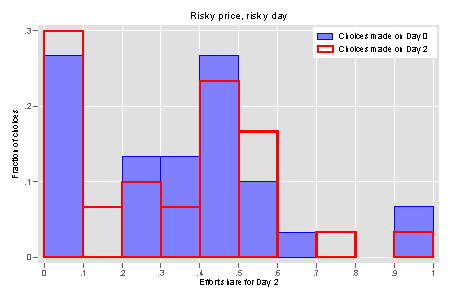
\includegraphics[width=\textwidth, trim=0cm 0cm 0cm 0cm, clip]{stata_graphics/effshare_hist_overlaid_rprd_3x2.pdf}
\end{frame}

\begin{frame}{Results: effort-share chosen at $R_2=1.25$ by treatment}
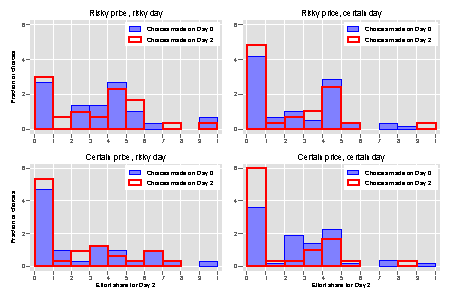
\includegraphics[width=\textwidth, trim=0cm 0cm 0cm 0cm, clip]{stata_graphics/effshare_hist_overlaid_bare_3x2.pdf}
\end{frame}

\begin{frame}{Results: treatment effects by day}
 \begin{center}
  \resizebox{0.65\textwidth}{!}{
  \begin{threeparttable}
    \begin{tabular}{lcc}
    \toprule
     & \multicolumn{2}{c}{Effort-share choices $\varphi_{i,d}$} \\ \cmidrule{2-3}
     & \multicolumn{1}{c}{On Day $d=0$} & \multicolumn{1}{c}{On Day $d=2$} \\
     \cmidrule(r){2-2} \cmidrule(l){3-3}
     Certain Price         & $-0.1747^{**}$  & $-0.2154^{***}$ \\
                           & $(0.0806)$      & $(0.0811)$      \\
     Certain Day           & $-0.0436 $      & $-0.0512 $      \\
                           & $(0.0368)$      & $(0.0493)$      \\
     Certain Price and Day & $ 0.0669 $      & $-0.0231 $      \\
                           & $(0.0908)$      & $(0.1166)$      \\
     $\ln R_i$             & $-0.6848^{***}$ & $-0.5907^{***}$ \\
                           & $(0.0738)$      & $(0.0869)$      \\
     Constant              & $ 0.4887^{***}$ & $ 0.4451^{***}$ \\
                           & $(0.0339)$      & $(0.0344)$      \\
     \cmidrule(r){2-2} \cmidrule(l){3-3}
     $N$ (Decisions) & \multicolumn{1}{c}{540} & \multicolumn{1}{c}{357} \\
     $G$ (Subjects)  & \multicolumn{1}{c}{180} & \multicolumn{1}{c}{121} \\
     \cmidrule(r){2-2} \cmidrule(l){3-3}
     $N_l$ (Left-censored)  & \multicolumn{1}{c}{ 92} & \multicolumn{1}{c}{ 68} \\
     $N_u$ (Uncensored)     & \multicolumn{1}{c}{391} & \multicolumn{1}{c}{257} \\
     $N_r$ (Right-censored) & \multicolumn{1}{c}{ 57} & \multicolumn{1}{c}{ 32} \\
    \bottomrule
    \end{tabular}
    \begin{tablenotes}[flushleft,para]
      \small \item \emph{Notes:} All attrited subjects are excluded. Standard errors are clustered on subject, using a two-limit Tobit regression model.
      \small \item[***] $p<0.01$
      \small \item[**]  $p<0.05$
      \small \item[*]   $p<0.10$
    \end{tablenotes}
  \end{threeparttable}
  }
 \end{center}
\end{frame}

\begin{frame}{Model}
\begin{itemize}[<+->]
\item Assume Expected Utility with Quasi-Hyperbolic Discounting (ANS 2015)
\item Simply compare present bias factor $\beta$ between treatments
\item CRRA periodic convex effort costs: $c(e) = (e + 10)^\alpha$

\item On decision-day $d$, minimize quasi-hyperbolic-discounted effort costs:
$$\min_{e_{i,d}^t} \beta^{\mathbbm{1}(d=0)}(e_{i,d}^\text{Day 2}+10)^\alpha + \beta \delta^7 (e_{i,d}^\text{Day 9}+10)^\alpha, \text{ s.t. } e_i^\text{Day 2} + R_i e_i^\text{Day 9} = 360$$

\item Euler equation:
$$\left( \frac{e_{i,d}^\text{Day 2}+10}{e_{i,d}^\text{Day 9}+10} \right)^{\alpha-1} = \frac{\beta^{\mathbbm{1}(d=2)} \delta^7}{R_i}$$

\item Reduced form:
$$ \underbrace{ \ln \frac{e_{i,d,s}^\text{Day 2}+10}{e_{i,d,s}^\text{Day 9}+10} }_{E_{i,d,s}} = \underbrace{ \frac{\ln \delta}{\alpha - 1} }_{\theta_{\textsf{delay}}} 7 + \underbrace{ \frac{-1}{\alpha - 1} }_{\theta_{\textsf{lnrate}}} \ln R_i + \underbrace{ \frac{\ln \beta}{\alpha - 1} }_{\theta_{\textsf{present}}} \mathbbm{1}(d=2) + \varepsilon_{i,d,s}$$
\item Recovery: $\alpha=1-\theta_{\textsf{lnrate}}^{-1}, \quad \beta=\exp(-\theta_{\textsf{present}}^{\strut}\theta_{\textsf{lnrate}}^{-1}), \quad \delta=\exp(-\theta_{\textsf{delay}}^{\strut}\theta_{\textsf{lnrate}}^{-1})$
\end{itemize}
\end{frame}

\begin{frame}{Model: pooled estimation}
\begin{itemize}[<+->]
\item Let's allow for different treatment-by-day effects:
\begin{align*}
 E_{i,d,s} &= \theta_{\textsf{delay}} 7 + \theta_{\textsf{lnrate}} \ln R_i + \theta_{\textsf{present}} \mathbbm{1}(\textsf{pr})_{d} + \theta_{\textsf{pr-cp}} \mathbbm{1}(\textsf{pr})_{d} \mathbbm{1}(\textsf{tr-cp})_{s} \\
 & \quad + \theta_{\textsf{pr-cd}} \mathbbm{1}(\textsf{pr})_{d} \mathbbm{1}(\textsf{tr-cd})_{s} + \theta_{\textsf{pr-cp-cd}} \mathbbm{1}(\textsf{pr})_{d} \mathbbm{1}(\textsf{tr-cp})_{s} \mathbbm{1}(\textsf{tr-cd})_{s} \\
 & \quad + \theta_{\textsf{tr-cp}} \mathbbm{1}(\textsf{tr-cp})_{s} + \theta_{\textsf{tr-cd}} \mathbbm{1}(\textsf{tr-cd})_{s} + \theta_{\textsf{tr-cp-cd}} \mathbbm{1}(\textsf{tr-cp})_{s} \mathbbm{1}(\textsf{tr-cd})_{s} + \varepsilon_{i,d,s}
\end{align*}
\item This will permit recovery of \alert{different $\beta$ and $\delta$} for each treatment:
\begin{align*}
  \alpha &= 1-\theta_{\textsf{lnrate}}^{-1} & & \\
  \delta_{\textsf{}} &= \exp \frac{\theta_{\textsf{delay}}}{-\theta_{\textsf{lnrate}}} & \delta_{\textsf{cp}} &= \exp \frac{\theta_{\textsf{delay}} + \theta_{\textsf{tr-cp}}}{-\theta_{\textsf{lnrate}}} \\
  \delta_{\textsf{cd}} &= \exp \frac{\theta_{\textsf{delay}} + \theta_{\textsf{tr-cd}}}{-\theta_{\textsf{lnrate}}} & \delta_{\textsf{cp-cd}} &= \exp \frac{\theta_{\textsf{delay}} + \theta_{\textsf{tr-cp}} + \theta_{\textsf{tr-cd}} + \theta_{\textsf{cp-cd}}}{-\theta_{\textsf{lnrate}}} \\
  \beta_{\textsf{}} &= \exp \frac{\theta_{\textsf{present}}}{-\theta_{\textsf{lnrate}}} & \beta_{\textsf{cp}} &= \exp \frac{\theta_{\textsf{present}} + \theta_{\textsf{pr-cp}}}{-\theta_{\textsf{lnrate}}} \\
  \beta_{\textsf{cd}} &= \exp \frac{\theta_{\textsf{present}} + \theta_{\textsf{pr-cd}}}{-\theta_{\textsf{lnrate}}} & \beta_{\textsf{cp-cd}} &= \exp \frac{\theta_{\textsf{present}} + \theta_{\textsf{pr-cp}} + \theta_{\textsf{pr-cd}} + \theta_{\textsf{pr-cp-cd}}}{-\theta_{\textsf{lnrate}}}
\end{align*}
\end{itemize}
\end{frame}

\begin{frame}{Results from restricted pooled model}
\begin{itemize}[<+->]
\item Restrict $\delta$ to be the same for all treatments
\item My \emph{ex ante} specification before seeing the data
\end{itemize}
\vspace{1\baselineskip}
\pause
\begin{columns}[T]
\begin{column}[c]{0.4\textwidth}
  \resizebox{1\textwidth}{!}{
    \begin{threeparttable}
      \begin{tabular}{lll}
        \toprule
        Param. $\theta$ & Estimate & $H_0\!\!: \theta=1$ \\
        \midrule
        $\beta_{\textsf{}}$       & $1.0069$ & $p=0.8965$ \\
        $\beta_{\textsf{cd}}$     & $0.9237$ & $p=0.1766$ \\
        $\beta_{\textsf{cp}}$     & $0.6822$ & $p=0.0033$ \\
        $\beta_{\textsf{cp-cd}}$  & $0.5833$ & $p=0.0001$ \\
        \midrule
        $\delta_{\textsf{}}$      & $0.9857$ & $p=0.0006$ \\
        \midrule
        $\alpha$                  & $1.2824$ & $p=0.0000$ \\
        \bottomrule
     \end{tabular}
    \begin{tablenotes}[para,flushleft]
      {\small \item \emph{Notes:} $N=897$ observations from $G=180$ clusters, with $N_l=160$ left- and $N_r=89$ right-censored observations. Standard errors are clustered on subject, using a two-limit Tobit regression model. }
    \end{tablenotes}
    \end{threeparttable}
  }
\end{column}%
\begin{column}[c]{0.6\textwidth}
  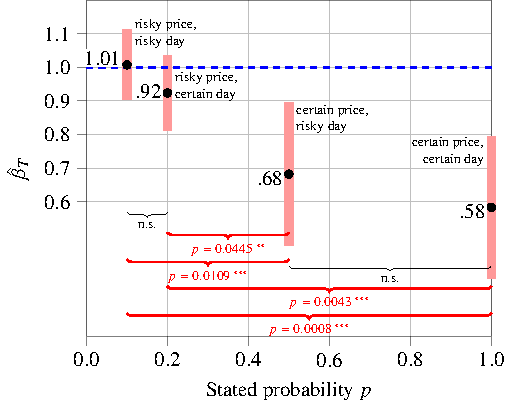
\includegraphics[width=\textwidth]{latex_figures/beta_by_treatment--stated_prob--restr.pdf}
\end{column}%
\end{columns}
\end{frame}

\begin{frame}{Results from unrestricted pooled model}
\begin{columns}[T]
\begin{column}[c]{0.4\textwidth}
  \resizebox{1\textwidth}{!}{
    \begin{threeparttable}
      \begin{tabular}{lll}
        \toprule
        Param. $\theta$ & Estimate & $H_0\!\!: \theta=1$ \\
        \midrule
        $\beta_{\textsf{}}$       & $0.9283$ & $p=0.0294$ \\
        $\beta_{\textsf{cd}}$     & $0.8978$ & $p=0.0558$ \\
        $\beta_{\textsf{cp}}$     & $0.8873$ & $p=0.2314$ \\
        $\beta_{\textsf{cp-cd}}$  & $0.6882$ & $p=0.0020$ \\
        \midrule
        $\delta_{\textsf{}}$      & $0.9970$ & $p=0.7603$ \\
        $\delta_{\textsf{cd}}$    & $0.9415$ & $p=0.3417$ \\
        $\delta_{\textsf{cp}}$    & $0.6822$ & $p=0.0136$ \\
        $\delta_{\textsf{cp-cd}}$ & $0.7461$ & $p=0.0157$ \\
        \midrule
        $\alpha$                  & $1.2824$ & $p=0.0000$ \\
        \bottomrule
     \end{tabular}
    \begin{tablenotes}[para,flushleft]
      {\small \item \emph{Notes:} $N=897$ observations from $G=180$ clusters, with $N_l=160$ left- and $N_r=89$ right-censored observations. Standard errors are clustered on subject, using a two-limit Tobit regression model. }
    \end{tablenotes}
    \end{threeparttable}
  }
\end{column}%
\begin{column}[c]{0.6\textwidth}
  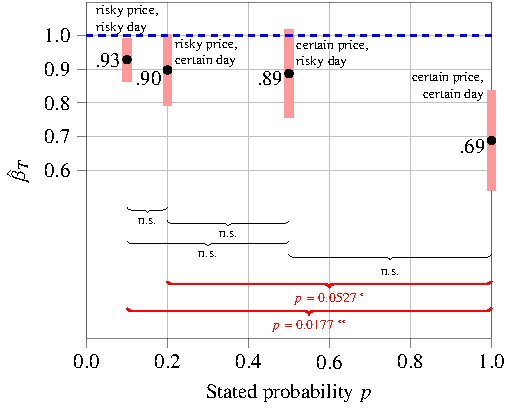
\includegraphics[width=\textwidth]{latex_figures/beta_by_treatment--stated_prob.pdf}
\end{column}%
\end{columns}
\vspace{1\baselineskip}
\pause
\begin{itemize}
\item Suggests a significant interaction between immediacy and certainty
\end{itemize}
\end{frame}

\begin{frame}{Results: attrition and continuation probability}
\begin{itemize}
\item Of subjects who completed Day 2, $93.75\%$ completed Day 9
\vspace{1\baselineskip}
\item Pooled estimate of $\hat{\delta^7}=90.39\%$, $95\%$ CI of $(85.15\%, 95.63\%)$
\vspace{1\baselineskip}
\item Fail to reject that subjects are sophisticated regarding their own attrition
\end{itemize}
\end{frame}


\begin{frame}{Model: within-subject estimation of $\beta_s$ and $\delta_s$}
\begin{itemize}[<+->]
\item Reduced form:
$$ \underbrace{ \ln \frac{e_{i,d,s}^\text{Day 2}+10}{e_{i,d,s}^\text{Day 9}+10} }_{E_{i,d,s}} = \underbrace{ \frac{\ln \delta_s}{\alpha - 1} }_{\theta_{\textsf{delay},s}} 7 + \underbrace{ \frac{-1}{\alpha - 1} }_{\theta_{\textsf{lnrate}}} \ln R_i + \underbrace{ \frac{\ln \beta_s}{\alpha - 1} }_{\theta_{\textsf{present},s}} \mathbbm{1}(d=2) + \varepsilon_{i,d,s}$$
\item Recovery: $\alpha=1-\theta_{\textsf{lnrate}}^{-1}, \quad \beta_s=\exp(-\theta_{\textsf{present},s}^{\strut}\theta_{\textsf{lnrate}}^{-1}), \quad \delta_s=\exp(-\theta_{\textsf{delay},s}^{\strut}\theta_{\textsf{lnrate}}^{-1})$
\end{itemize}
\end{frame}

\begin{frame}{Results: within-subject estimation of $\beta_s$}
 \begin{center}
    \begin{tabular}{lrr}
    \toprule
    \multicolumn{3}{c}{Number of subjects with $\hat\beta_s<1$} \\
    \midrule
        Treatment & \hspace{1em} Risky Day & \hspace{1em} Certain Day \\
    \midrule
      Risky Price &  15 of 29 &    12 of 29 \\
    Certain Price &   7 of 30 &     9 of 29 \\
    \bottomrule
    \end{tabular}
 \end{center}
\end{frame}

\begin{frame}{Results: within-subject estimation of $\beta_s$}
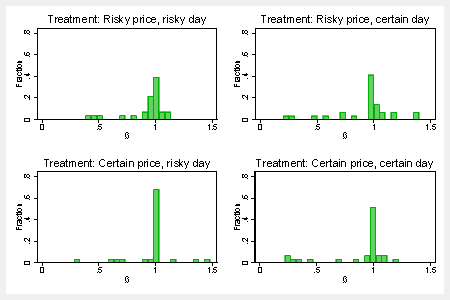
\includegraphics[width=\textwidth, trim=0.2cm 0.3cm 0.2cm 0.2cm, clip]{stata_graphics/beta_hist--2x2.pdf}
\end{frame}

\begin{frame}{Result robustness}
$$E_{i,d} \coloneqq \ln\frac{e_{i,d}^\text{Day 2}+\omega}{e_{i,d}^\text{Day 9}+\omega}, \quad \text{with background effort} \;\; \omega$$\\
\begin{itemize}[<+->]
\item Results for various levels of background effort give similar results \\
\item Levels of $\omega$ validated: $10$, $100$, $1\,000$, $10\,000$
\vspace{3\baselineskip}
\item All regressions show significant convexity in effort-cost
\item On average, subjects prefer to smooth effort between days
\end{itemize}
\end{frame}

\begin{frame}
\vfill
\begin{center}
{\Large Conclusion}
\end{center}
\vfill
\end{frame}

\begin{frame}{What have I shown?}
\begin{itemize}[<+->]
\item \alert{Clear evidence that present bias is diminished by uncertainty}
\vspace{1\baselineskip}
\item The extent of present-biasedness seems roughly unaffected
\vspace{1\baselineskip}
\item Present bias is attenuated by two types of risk:
\begin{itemize}[<+->]
\item Risk between decisions made on different days \\ \textcolor{gray}{ (implies dynamic inconsistency) }
\item Risk between decisions made at different prices \\ \textcolor{gray}{ (standard probability weighting) }
\end{itemize}
\vspace{1\baselineskip}
\item Slightly underpowered to find differences for intermediate levels of risk
\end{itemize}
\end{frame}

\begin{frame}{Implications}
\begin{itemize}[<+->]
\item Risk and time preferences: a foundation of microeconomics
\begin{itemize}[<+->]
\item Supports recent theory linking certainty and immediacy\\
\textcolor{gray}{Baucells and Heukamp (2012); Epper and Fehr-Duda (2018); Chakraborty, Halevy, and Saito (2020)}
\end{itemize}
\vspace{1\baselineskip}
\item Implications for worker behavior:
\begin{itemize}[<+->]
\item Ride-hail drivers' labor supply may be significantly affected by risk
\item Uncertainty regarding wage rate or ride length may affect procrastination
\end{itemize}
\vspace{1\baselineskip}
\item Implications for consumer behavior:
\begin{itemize}[<+->]
\item Savings and spending behavior may be affected by risk
\item Temptation goods' value may be affected by risk
\end{itemize}
\vspace{1\baselineskip}
\item Implications for economic methodology:
\begin{itemize}[<+->]
\item Beware of decision risk confounding measures of present bias
\end{itemize}
\end{itemize}
\end{frame}

\begin{frame}{Ongoing research}
\begin{itemize}[<+->]
\item Test the probability-delay rank-dependent utility model
\begin{itemize}
\item \textcolor{gray}{Baucells and Heukamp (2012)}
\item \textcolor{gray}{Epper and Fehr-Duda (2018)}
\item \textcolor{gray}{Chakraborty, Halevy, and Saito (2020) }
\end{itemize}
\vspace{1\baselineskip}
\item Are the present-biased decision-makers also non-EUT?
\vspace{1\baselineskip}
\item Disentangle complexity from risk and time preferences
\begin{itemize}
\item \textcolor{gray}{Bernheim and Sprenger (2020) }
\end{itemize}
\end{itemize}
\end{frame}

\begin{frame}
\vfill
\begin{center}
{\Large Thank you!} \\
\vspace{1\baselineskip}
Please send any comments to \texttt{reddinger@ucsb.edu}
\end{center}
\vfill
\end{frame}

\end{document}
